\chapter{Pythagorean Theorem}

If you have a right triangle, the edges that touch the right angle are
called \emph{the legs}.  The third edge is known as \emph{the
  hypotenuse}. The Pythagorean Theorem gives us the relationship
between the length of the legs and the length of the hypotenuse.

\begin{tikzpicture}[scale=1.2]
  \coordinate [circle, fill, inner sep=1pt] (a) at (0,0) ;
  \coordinate [circle, fill, inner sep=1pt] (b) at (0,4) ;
  \coordinate [circle, fill, inner sep=1pt] (c) at (3,0) ;
  \draw (a)--node [outer sep=3pt, left]{Length $a$}(b);
  \draw (b)--node[outer sep=3pt, right]{Length $c$}(c) ;
  \draw (c)--node[outer sep=3pt, below]{Length $b$}(a) ;
  \pic [draw, angle eccentricity=1.5] {right angle = c--a--b};
\end{tikzpicture}

The Pythagorean Theorem tells us that $a^2 + b^2 = c^2$.

For example, if one leg has length 3 and the other has length 4, then
$a^2 + b^2 = 3^2 + 4^2 = 25$. Thus $c^2$ must equal 25. So you know
the hypotenuse must be of length 5.

(In reality, it almost never works out to be such a tidy number. For
example, what is the length of the hypotenuse if the two legs are 3
and 6? $a^2 + b^2 = 3^2 + 6^2 = 45$.  The length of the hypotenuse is
the square root of that: $\sqrt{45} = \sqrt{9 \times 5} = 3 \sqrt{5}$,
which is approximately 6.708203932499369.)

\section{Distance between Points}

What is the distance between these two points?

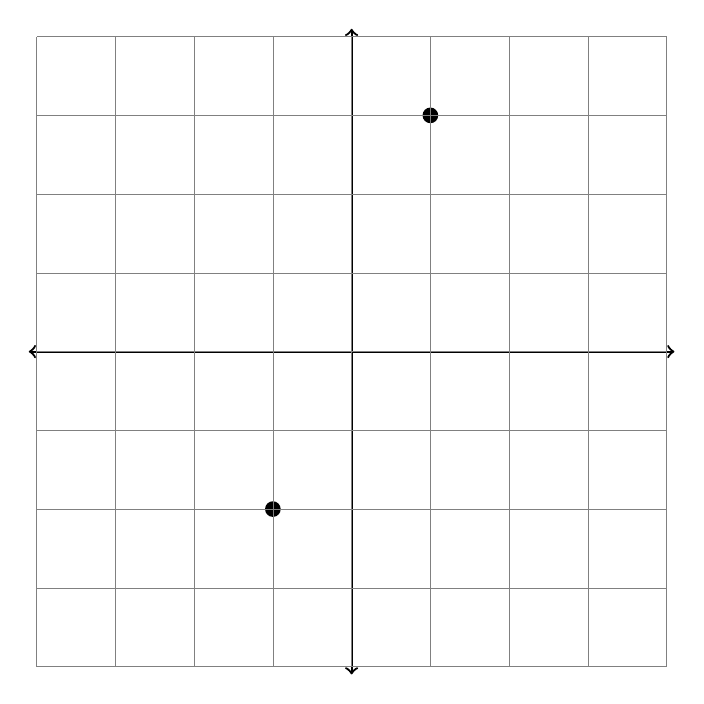
\begin{tikzpicture}
  % axis
  \draw[thick, <->] (0, -4.1) -- (0, 4.1);
  \draw[thick, <->] (-4.1, 0) -- (4.1, 0);
  \coordinate [circle, fill, inner sep=2pt] (a) at (-1,-2) ;
  \coordinate [circle, fill, inner sep=2pt] (a) at (1,3) ;

  % grid
  \draw[help lines, step = 1cm] (-4, -4) grid (4, 4);
  
\end{tikzpicture}

We can draw a right triangle and use the Pythagorean Theorem:

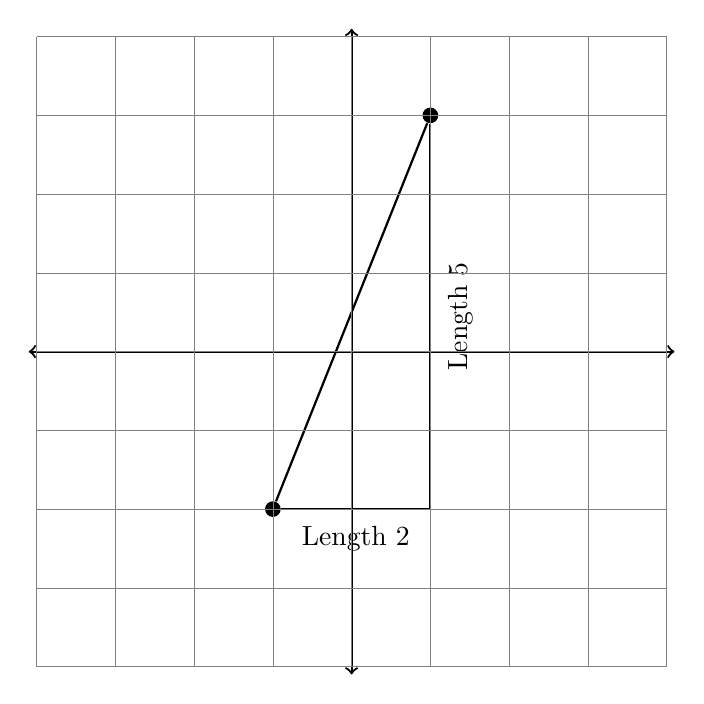
\begin{tikzpicture}
  % axis
  \draw[thick, <->] (0, -4.1) -- (0, 4.1);
  \draw[thick, <->] (-4.1, 0) -- (4.1, 0);
  \coordinate [circle, fill, inner sep=2pt] (a) at (-1,-2) ;
  \coordinate [circle, fill, inner sep=2pt] (b) at (1,3) ;
  \coordinate (c) at (1, -2);

  \draw [thick] (a) -- (b);
    \draw [thick] (a) -- node[outer sep = 3pt, below]{Length 2}(c);
      \draw [thick] (c) -- node[rotate=90, outer sep = 3pt, below]{Length 5}(b);
  \draw[help lines, step = 1cm] (-4, -4) grid (4, 4);
 
\end{tikzpicture}

The distance between the two points is $\sqrt{2^2 + 5^2} = \sqrt{29} \approx 5.385165$.
